%!TEX root = principal.tex
\section{Ladder e Instruction List}

Apesar de parecer com um circuito, um diagrama ladder é a descrição de um código, executado da esquerda para a direita e de cima para baixo. Na prática, o ladder tem uma estrutura muti parecida com o Instruction List, portanto é interessante compararmos os 2.

Para o funcionamento do ladder ou de IL, o CLP trabalha com uma estrutura chamada pilha, que é uma memória do tipo LIFO -- \emph{last in, first out}, que pode ser visualizada como uma pilha de papel, onde o último papel colocado é o primeiro retirado. A pilha tem duas funções básicas de acesso: a load (LD), que carrega um dado de alguma posição de memória para o topo da pilha, e a store (ST), que armazena a informação no topo da pilha em alguma posição de memória. Estas posições de memória podem ser memórias internas, entradas ou saídas de um CLP. Pos simplicidade, chamemos o topo da pilha de acumulador.

Na linguagem IL, as instruções lidam diretamente com o acumulador, que passa a funcionar como uma variável implícita. Por exemplo: um código IL que define uma saída como o E de duas entradas é simplesmente:
\begin{lstlisting}[caption=Código IL de um E lógico, label=lst:andIL]
LD %I0
AND %I1
ST %Q0
\end{lstlisting}

No código \ref{lst:andIL}, a instrução \lstinline|LD %I0| carrega a entrada 0 no acumulador. Logo depois a instrução \lstinline|AND %I1| faz o E lógico do valor na entrada 1 com o valor no acumulador (que foi copiado da entrada 0) e guarda o resultado no próprio acumulador. É como se retirasse o valor da pilha, fizesse a operação, e guardasse de volta na pilha. Agora o acumulador contém o resultado do E lógico entre \lstinline|%I0| e \lstinline|%I1|. Por último, a instrução \lstinline|ST %Q0| passa o valor no acumulador para a saída 0.

Este código é equivalente ao ladder da figura \ref{fig:ladder_AND}. Neste caso, o primeiro contato carrega a entrada 0 no acumulador. Como o segundo contato está em série, ele equivale à AND do IL. A bobina então salva o valor presente no acumulador na saída 0. Note-se então a relação que há entre a bobina do ladder e o comando ST do IL e entre o contato do ladder e os comandos LD, AND e OR do IL. Não é então de se admirar que se tenha o equivalente aos contatos normalmente fechados em IL -- basta acrescentar um N aos comandos IL: LDN, STN, ANDN, ORN.

\begin{figure}[hbt]
	\centering
	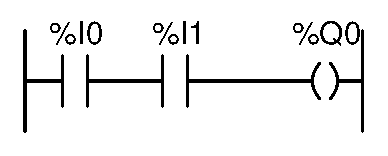
\includegraphics[scale=0.6]{figuras/ladder_AND}
	\caption{Ladder equivalente ao IL do código \ref{lst:andIL}.}
	\label{fig:ladder_AND}
\end{figure}

A pilha acaba sendo usada quando se tem caminhos paralelos no ladder. Analise-se por exemplo o ladder da figura \ref{fig:ladder_ABorCD}. Um compilador ladder, analisando o diagrama da esquerda para a direita, vai carregar A, fazer o AND com B e, chegando à junção, checar de onde ela se origina, ele então vai carregar C, no topo da pilha acima do resultado do AND entre A e B que já está lá, fazer o AND com D, então fazer o OR entre os dois valores no topo da pilha e salvar o resultado em X. Um código IL equivalente é mostrado ao lado do ladder. Observe no IL que neste caso o comando OR não tem nenhum argumento; o que faz com que ele execute a operação com os dois últimos valores da pilha.

\newsavebox\ladderABorCD
\begin{lrbox}{\ladderABorCD}
\begin{minipage}[b]{0.3\textwidth}
\begin{lstlisting}
LD A
AND B
LD C
AND D
OR
ST X
\end{lstlisting}
\end{minipage}
\end{lrbox}

\begin{figure}[hbt]
	\centering
	\subfloat[ladder]{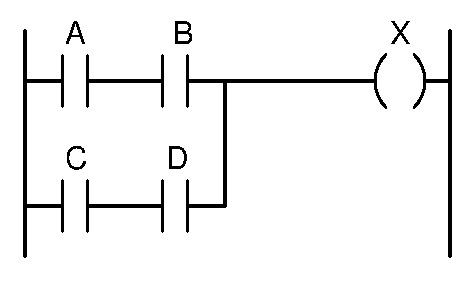
\includegraphics[scale=0.6]{figuras/ladder_ABorCD}}
	\qquad\qquad
	\subfloat[IL]{\centering\usebox{\ladderABorCD}
	}
	\caption{Exemplo de ladder e IL que usa a pilha para armazenar um valor intermediário.}
	\label{fig:ladder_ABorCD}
\end{figure}


\section{Memória}
É possível no ladder, assim como também o é usando relês, acionar uma bobina X com uma lógica que usa o contato X. Isto gera uma realimentação que tem umas propriedades interessantes. Veja por exemplo o ladder e equivalente IL da figura \ref{fig:ladder_latch}.

\newsavebox\mybox
\begin{lrbox}{\mybox}
\begin{minipage}[b]{0.3\textwidth}
\begin{lstlisting}[]
LD %I0
OR %M0
ANDN %I1
ST %M0
\end{lstlisting}
\end{minipage}
\end{lrbox}


\begin{figure}[hbt]
	\centering
	\subfloat[ladder]{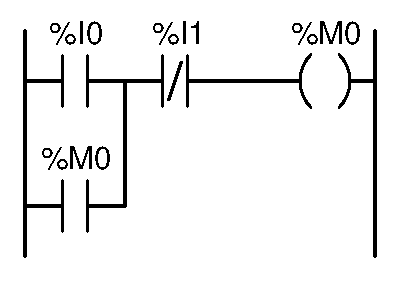
\includegraphics[scale=0.6]{figuras/ladder_latch}}
	\qquad\qquad
	\subfloat[IL]{\centering\usebox{\mybox}
	}
	\caption{Ladder e IL implementando um latch.}
	\label{fig:ladder_latch}
\end{figure}

Esta estrura faz com que, se \%I0 for acionado, aciona-se \%M0, que fica acionado daí por diante independente de \%I0. \%M0 só deixa de ser acionado se for acionado \%I1. Isto faz com que \%M0 implemente uma memória de 1 bit. Esta estrutura é a base inicial das primeiras memórias de computadores eletromecânicos e é chamada de latch. Neste caso \%I0 funciona como o sinal de SET e \%I1 como o reset deste latch.

Por ser muito útil, a funcionalidade de latch acaba sendo criado diretamente, pelos comandos de set (S em IL e 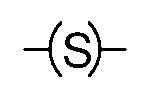
\includegraphics[height=0.9em]{figuras/bobina_S} em ladder) e reset, (R em IL e 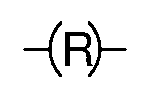
\includegraphics[height=0.9em]{figuras/bobina_R} em ladder). Estes comandos fazem com que o exemplo da figura \ref{fig:ladder_latch} possa ser implementado mais facilmente, como mostra a figura \ref{fig:ladder_latchSR}.
\newsavebox\latchSRbox
\begin{lrbox}{\latchSRbox}
\begin{minipage}[b]{0.3\textwidth}
%\vspace{0pt}
\begin{lstlisting}[]
LD %I0
S %M0
LD %I1
R %M0
\end{lstlisting}
\end{minipage}
\end{lrbox}


\begin{figure}[hbt]
	\centering
	\subfloat[t][ladder]{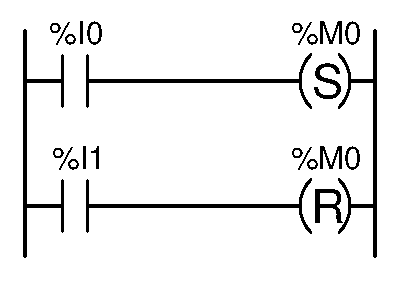
\includegraphics[scale=0.6]{figuras/ladder_latchSR}}
	\qquad\qquad
	\subfloat[t][IL]{\centering\usebox{\latchSRbox}
	}
	\caption{Ladder e IL implementando um latch com os comandos de set e reset.}
	\label{fig:ladder_latchSR}
\end{figure}

\subsection{Subida e descida de uma entrada.}

Considere que se queira inverter uma saída cada vez que se aperte um botão. A princípio bastaria fazer o ladder da figura \ref{fig:ladder_pulsoRuim}, que ao apertar o botão, seta a saída se ela estiver 0 ou reseta se estiver 1. Porém esta solução não funciona, pois a cada ciclo a situação da saída estará trocada e ela vai acabar oscilando enquanto a chave estiver pressionada.

\begin{figure}[hbt]
	\centering
	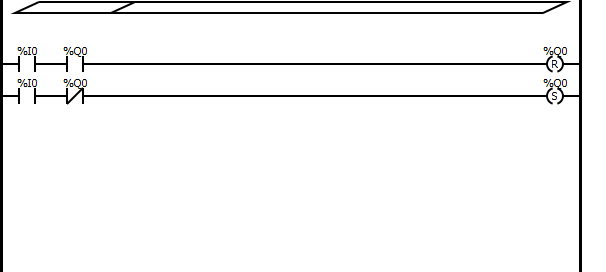
\includegraphics[width=\textwidth]{figuras/pulsoRuim}
	\caption{Troca de saída ao apertar um botão -- solução errada.}
	\label{fig:ladder_pulsoRuim}
\end{figure}

É necessário então um modo de garantir a inversão da saída apenas da primeira vez que se detecta o botão apertado. Isto pode ser conseguindo armazenando o botão numa variável auxiliar \emph{apenas ao final} do ciclo. Deste modo a variável auxiliar vai armazenar a entrada \emph{antiga}, do ciclo anterior. Com isto podemos detectar a subida da entrada se a entrada estiver acionada mas sua cópia antiga não estiver. Isto é feito na figura \ref{fig:ladder_pulso}.
\begin{figure}[hbt]
	\centering
	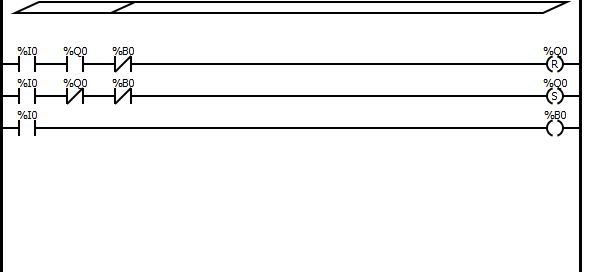
\includegraphics[width=\textwidth]{figuras/pulso}
	\caption{Troca de saída ao apertar um botão -- solução correta.}
	\label{fig:ladder_pulso}
\end{figure}

A norma define um comando específico para ladder nesta situação, que é acionado apenas no primeiro ciclo que a variável é acionada. Este comando é identificado por um contato com um P no meio, muito embora o classicladder use um chapeuzinho, identificando a subida do sinal. Também há um comando específico para determinar a descida de um sinal, indicado ou por um N no meio do contato ou por um chapeuzinho descendo, no caso do classicladder.

\begin{figure}[hbt]
	\centering
	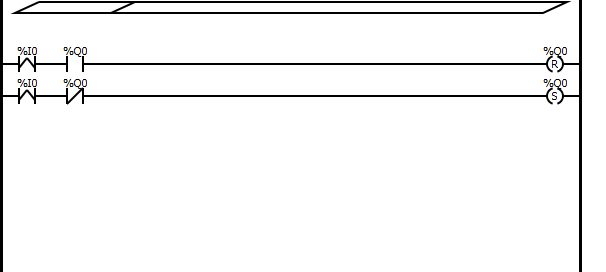
\includegraphics[width=\textwidth]{figuras/pulso2}
	\caption{Troca de saída ao apertar um botão usando o detetor de subida.}
	\label{fig:ladder_pulso2}
\end{figure}
